\documentclass[tikz, border=5pt]{standalone}
\usepackage{amsmath}
\usetikzlibrary{matrix, positioning, decorations.pathreplacing, calc}

\begin{document}
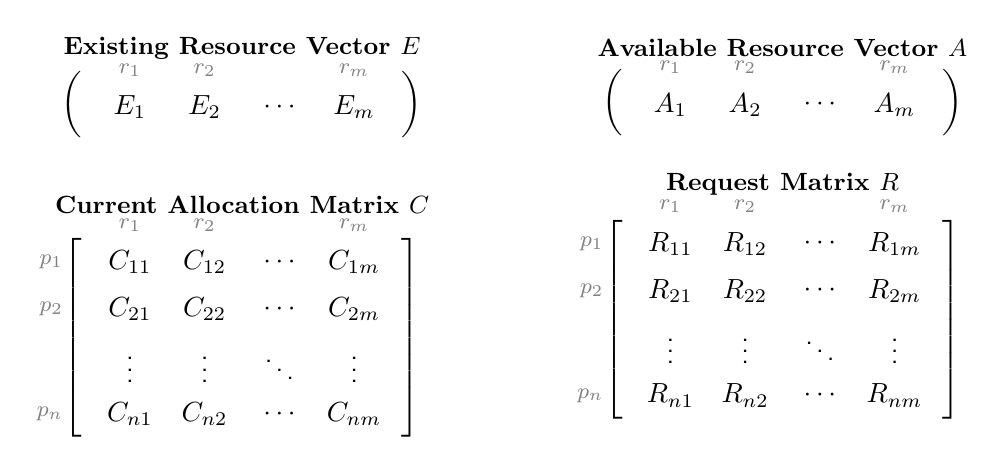
\begin{tikzpicture}[
    font=\sffamily,
    >=stealth,
    % Styles
    matrix_node/.style={matrix of math nodes, nodes={minimum width=2.5em, minimum height=1.5em, anchor=center, inner sep=2pt}, column sep=0.2em, row sep=0.2em},
    bracket_matrix/.style={matrix_node, left delimiter={[}, right delimiter={]}},
    paren_vector/.style={matrix_node, left delimiter={(}, right delimiter={)}},
    label_text/.style={font=\bfseries\small, align=center, anchor=south},
    row_label/.style={font=\footnotesize\color{gray}, anchor=east, xshift=-0.8em},
    col_label/.style={font=\footnotesize\color{gray}, anchor=south}
]

% 1. Existing Resource Vector E
\node[label_text] (lbl_E) {Existing Resource Vector $E$};
\matrix[paren_vector, below=0.1cm of lbl_E] (mat_E) {
    E_1 & E_2 & \cdots & E_m \\
};

% 2. Available Resource Vector A
\node[label_text, right=2cm of lbl_E] (lbl_A) {Available Resource Vector $A$};
\matrix[paren_vector, below=0.1cm of lbl_A] (mat_A) {
    A_1 & A_2 & \cdots & A_m \\
};

% 3. Current Allocation Matrix C
\node[label_text, below=1.5cm of lbl_E] (lbl_C) {Current Allocation Matrix $C$};
\matrix[bracket_matrix, below=0.1cm of lbl_C] (mat_C) {
    C_{11} & C_{12} & \cdots & C_{1m} \\
    C_{21} & C_{22} & \cdots & C_{2m} \\
    \vdots & \vdots & \ddots & \vdots \\
    C_{n1} & C_{n2} & \cdots & C_{nm} \\
};

% 4. Request Matrix R
\node[label_text] (lbl_R) at (lbl_A |- lbl_C) {Request Matrix $R$};
\matrix[bracket_matrix, below=0.1cm of lbl_R] (mat_R) {
    R_{11} & R_{12} & \cdots & R_{1m} \\
    R_{21} & R_{22} & \cdots & R_{2m} \\
    \vdots & \vdots & \ddots & \vdots \\
    R_{n1} & R_{n2} & \cdots & R_{nm} \\
};

% Annotations
% Resources labels (Columns)
\foreach \col/\label in {1/1, 2/2, 4/m} {
    \node[col_label] at (mat_E-1-\col.north) {$r_{\label}$};
    \node[col_label] at (mat_A-1-\col.north) {$r_{\label}$};
    \node[col_label] at (mat_C-1-\col.north) {$r_{\label}$};
    \node[col_label] at (mat_R-1-\col.north) {$r_{\label}$};
}

% Processes labels (Rows)
\foreach \row/\label in {1/1, 2/2, 4/n} {
    \node[row_label] at (mat_C-\row-1.west) {$p_{\label}$};
    \node[row_label] at (mat_R-\row-1.west) {$p_{\label}$};
}

\end{tikzpicture}
\end{document}
